\centerline{\bf \Large  4 класс}

\problem{\textbf{1}} Пюрвя Мучкаевич придумал систему перевода цифр в буквы и обратно, в которой каждой из десяти цифр соответствует одна уникальная буква. Он решил воспользоваться новой системой и сложил в столбик два слова УДЕ + УДЕ. Мог ли Пюрвя Мучкаевич получить в результате слово НАУКА? Если мог, то приведите пример таких чисел, если нет, то объясните почему.

\textbf{Решение:} Не мог получить пятизначное. Заметим, что сумма двух трёхзначных чисел не может быть больше четырёхзначного числа, т.к. максимально можно получить 999 + 999 = 1998. 

\textbf{Критерии.} \\
\textit{7 баллов} $-$ Полностью верное решение\\
\textit{5 баллов} $-$ Невозможность из-за суммы, которая может быть максимально четырёхзначной\\
\textit{0-2 балла} $-$ Доказательство того, что максимальная сумма четырёхзначная\\
\textit{0 баллов} $-$ Любое решение, в котором мог\\
\textit{0 баллов} $-$ Любой ответ без объяснений\\

\problem{\textbf{2}} Решите задачу:

а) Батыр и Очир вместе решают сборник 720 удивительных заданий Пюрви Мучкаевича за 40 дней. За сколько дней решит этот сборник один Батыр, если он за 4 дня решает столько же заданий, сколько Очир за 5 дней?

б) Составьте и решите обратную задачу по схеме: 720; ?; 72; 4; 5.

\textbf{Решение А:} Вместе решают 720/40=18 заданий в день. Если Батыр решает 10 заданий, а Очир 8, то условие задания выполняется. Батыр решит весь сборник за 720/10=72 дня.

\textbf{Примерное условие Б:} Батыр решает сборник 720 удивительных заданий Пюрви Мучкаевича за 72 дня. За сколько дней решат этот сборник Батыр вместе с Очиром, если Батыр за 4 дня решает столько же заданий, сколько Очир за 5 дней?

\textbf{Решение Б:} Батыр решает 720/72=10 заданий в день. За 4 дня решит 4$\cdot$10=40 заданий. Очир за один решает 40/5=8 заданий. Вместе решают 10+8=18 заданий в день. Вместе решат весь сборник за 720/18=40 дней.

\textbf{Критерии.} \\
\textit{0-4 баллов} $-$ Решение пункта А\\
\textit{0-1 балла} $-$ Составление условия пункта Б \\
\textit{0-2 баллов} $-$ Решение пункта Б\\
\textit{0 баллов} $-$ Любой ответ без объяснений\\

\problem{\textbf{3}} В степи паслись 25 коров. Пастухи пригнали стадо овец. Овец оказалось больше, чем у коров ушей, но меньше, чем у коров ног. Сколько было овец, если их в 25 раз больше, чем пастухов?

\textbf{Решение:} Овец больше 2$\cdot$25=50, но меньше 4$\cdot$25=100. При этом число овец кратно 25, т.к. их в 25 раз больше, чем пастухов (число которых является натуральным). Следовательно, овец 75.

\textbf{Критерии.} \\
\textit{1 балл} $-$ 2$\cdot$25=50\\
\textit{1 балл} $-$ 4$\cdot$25=100\\
\textit{2 балла} $-$ Количество овец больше 50 и меньше 100\\
\textit{3 балла} $-$ Количество овец кратно 25\\
\textit{0 баллов} $-$ Любой ответ без объяснений\\

\problem{\textbf{4}} Разрежьте фигуру, изображённую на рисунке снизу, по клеточкам на три
нераспадающиеся части так, чтобы из них можно было сложить квадрат (поворачивать части можно, переворачивать нельзя).

\begin{center}
    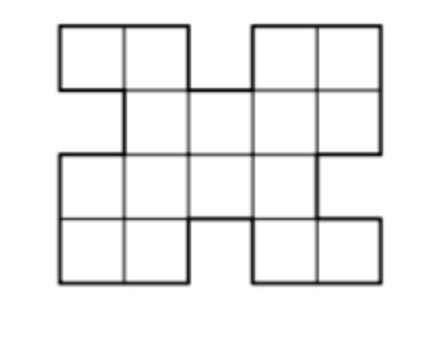
\includegraphics[width=0.2\textwidth]{Секретная информация/УДЕ 2024-2025/Регион. Условия/4.4.png}
\end{center}

\textbf{Решение:} 

\begin{center}
    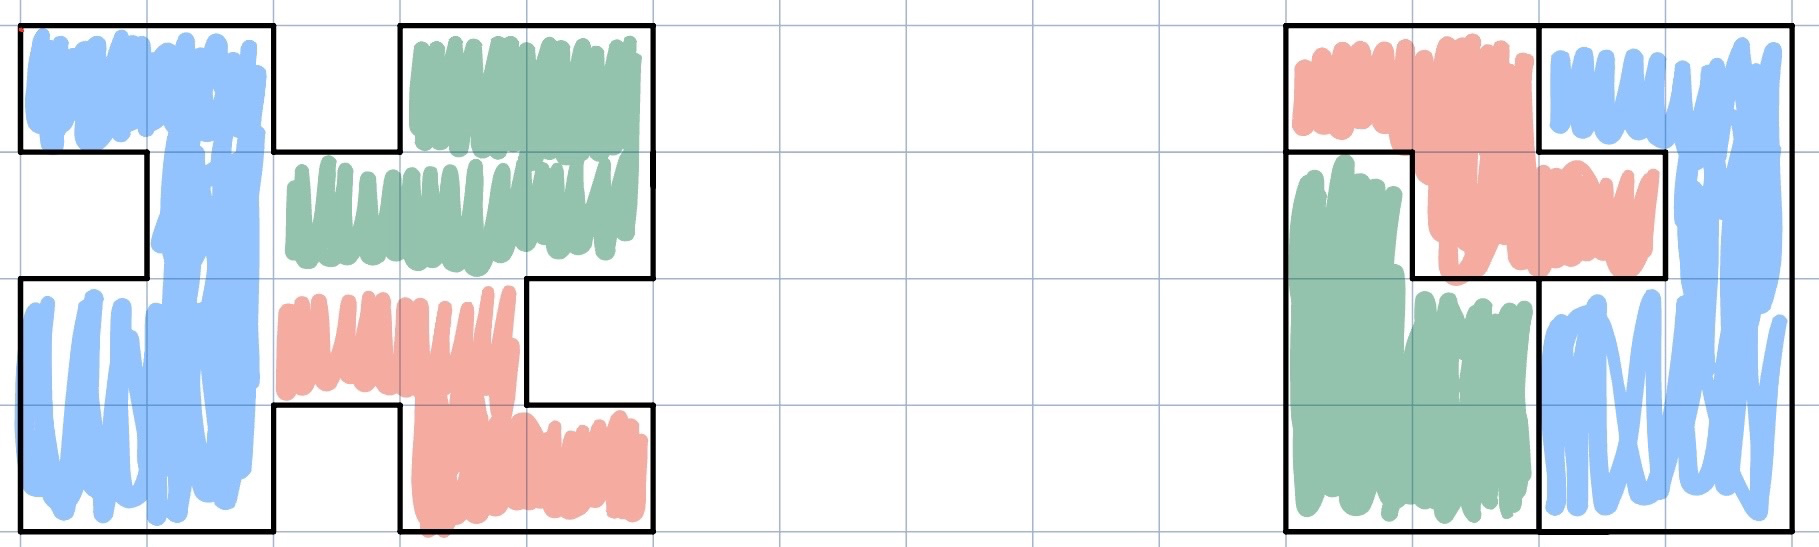
\includegraphics[width=0.4\textwidth]{Секретная информация/УДЕ 2024-2025/Регион. Решения/4.4_sol.png}
\end{center}

\textbf{Критерии.} \\
\textit{7 баллов} $-$ Любой правильный пример\\
\textit{3 балла} $-$ За понимание сложить квадрат 4$\times$4 из-за площади\\
\textit{0 баллов} $-$ Любой неправильный пример\\

\problem{\textbf{5}} Фигура \textit{Сайгак} бьёт все клетки, находящиеся от неё через клетку слева, справа, сверху или снизу, а также бьёт клетку, на которой стоит. Какое наименьшее количество \textit{Сайгаков} необходимо поставить на клетчатую доску 8 × 8 , чтобы эти фигуры били все клетки доски?

\textbf{Решение:} Раскрасим клетки доски в 4 цвета следующим образом: все клетки, куда может прийти Сайгак из, не умаляя общности, левой нижней угловой клетки, покрасим в первый цвет. Сдвигами этого множества клеток вправо, вверх и вправо вверх получаем 4 множества клеток. Рассмотрим одно из них. Чтобы все клетки были побиты, нужно как минимум 4 Сайгака, так как каждый из них бьёт не более 5   клеток, и, следовательно, 3 и меньше Сайгаков бьют максимум 15 клеток. Пример расстановки 4   Сайгаков: выделим 4  непересекающихся Т-образных фигур, в каждой из которых отметим по одному Сайгаку. И так как Сайгак, стоящий на клетке из одного множества, не может дойти до клеток из трёх других, получаем, что всего нужно как минимум 16 Сайгаков.

\begin{center}
    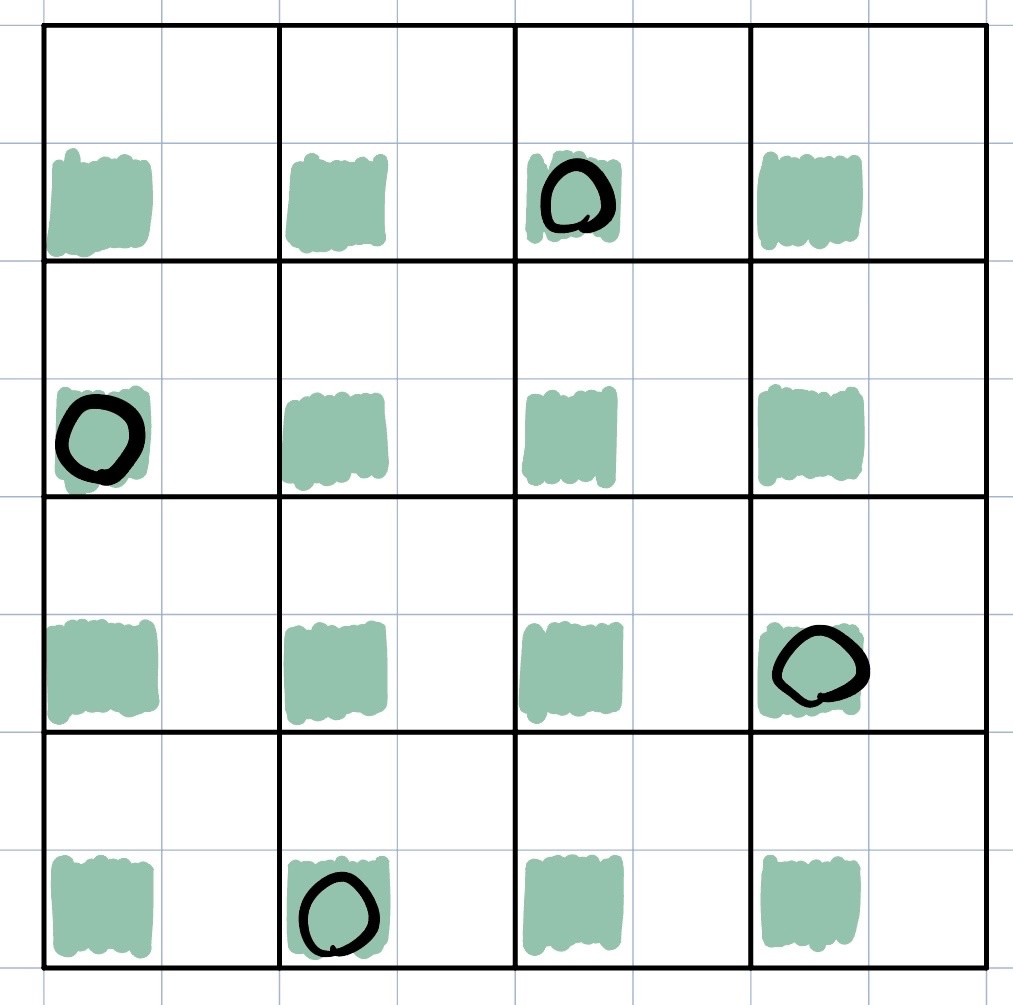
\includegraphics[width=0.3\textwidth]{Секретная информация/УДЕ 2024-2025/Регион. Решения/4.5_5.4_6.3.png}
\end{center}

\textbf{Критерии.} \\
\textit{2 балла} $-$ 16 Сайгаков без объяснений\\
\textit{1 балл} $-$ Меньше 16 Сайгаков без объяснений\\
\textit{0 баллов} $-$ Больше 16 Сайгаков без объяснений\\
\textit{0-5 баллов} $-$ Поиск примера и оценка\\